\subsection{Hits and clusters}
\label{HtsClstrs}

A track passing through a particular doublet layer produces scintillation light in one or at most two fibre channels. For each channel ``hit'', the tracker data acquisition system records the channel number, $n$, and the pulse height. After calibration, the pulse height is recorded in terms of the number of photo-electrons ($n_{\rm pe}$) generated in the Visible Light Photon Counter (VLPC) illuminated by the hit channel. Occasionally, showers of particles or noise can cause three or more neighbouring channels to be hit. The term ``clusters'' is used to refer to an isolated hit, a doublet cluster and a multi-hit cluster.

The position of a hit in the doublet-layer coordinate system may be determined from the channel number. For isolated hits, the measured coordinate $\alpha \in {u, v, w}$ is given by:

\begin{equation}
  \alpha = c_p (n - n_0)\,;
\end{equation}
where $n_0$ is the channel number of the central fibre and $c_p$ is the channel pitch given by:

\begin{equation}
  c_p = 3f_p + f_d
\end{equation}
where $f_d$ is the fibre diameter ($f_d = 350\,\mu{\rm m}$) and $f_p = $ is the fibre pitch ($f_p = 427\,\mu{\rm m}$ see figure~\ref{Fig:DblLyr}). For clusters in which two channels are hit (``doublet clusters'', see figure~\ref{Fig:Clust}), the measured coordinate is given by:

\begin{equation}
  \alpha = c_p \left[ \frac{( n_1 + n_2)}{2} - n_0 \right]\,;
\end{equation}
where $n_1$ and $n_2$ are the channel numbers of the two hit fibres. For a multi-hit cluster (clusters with more than two neighbouring channels), the measured position is determined from the pulse-height weighted mean of the fibre positions:

\begin{equation}
  \alpha = c_p \left[ 
                 \frac{\sum_i n_{{\rm pe}i}n_i}{\sum_i n_{{\rm pe}i}} 
               \right]\,;
\end{equation}
where the subscript $i$ indicates the $i^{\rm th}$ channel. The pulse-height for doublet and multi-channel clusters is determined by summing the pulse height of all the hits that make up the cluster.

\begin{figure}
  \begin{center}
    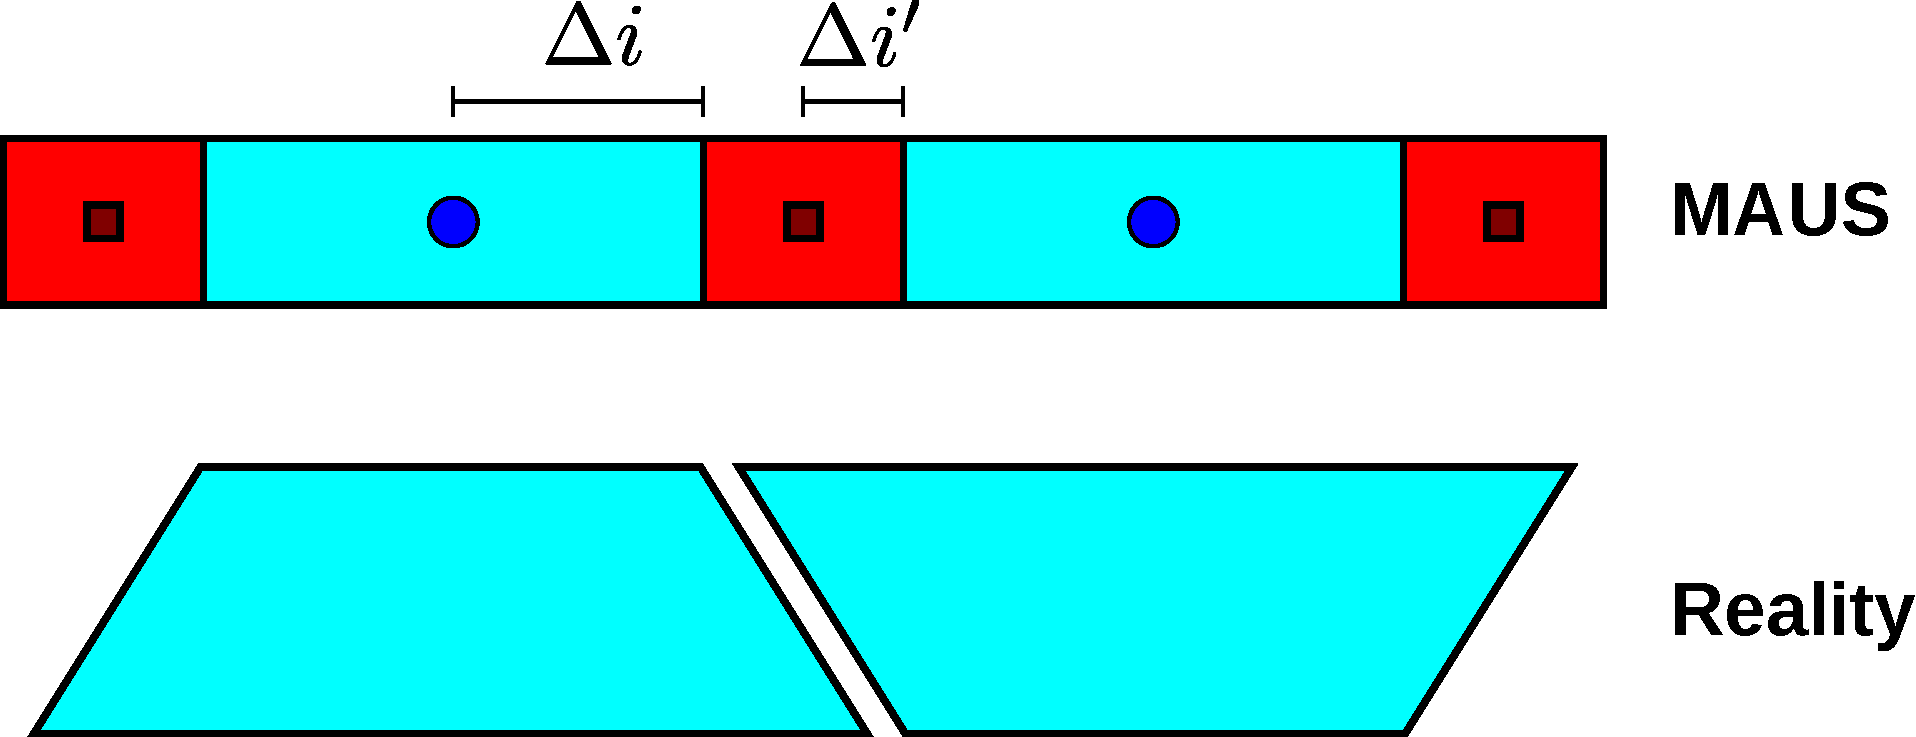
\includegraphics[width=0.9\linewidth]{detectors/tracker/04-Reconstruction/04-01-Hits-and-clusters/Figures/cluster-resolution.pdf}
  \end{center}
  \caption{Channel overlap as simulated in MAUS; fine-tuning reduces the error associated to doublet clusters.} 
  \label{Fig:Clust}
\end{figure}
The ``measurement vector'', ${\bf m}$ is defined as:

\begin{equation}
  {\bf m} =  \left( 
               \begin{array}{c}
                 \alpha \\ \beta
               \end{array}
              \right) \, ;
\end{equation}
where $\alpha$ is given above and, in the absence of additional information, $\beta = 0$. The corresponding covariance matrix is given by:

\begin{equation}
  \underline{\underline{V_m}} = 
    \left( 
      \begin{array}{cc}
         \sigma^2_\alpha & 0         \\
         0          & \sigma^2_\beta \\
       \end{array}
     \right) \, ;
\end{equation}
where $\sigma^2_\alpha$ and $\sigma^2_\beta$ are the variance of $\alpha$ and $\beta$ respectively. The variance on $\alpha$ for a single-hit cluster is given by:

\begin{equation}
  \sigma^2_m = \frac{c^2_p}{12} \, .
\end{equation}
For a doublet-cluster, the variance is given by:

\begin{equation}
  \sigma^2_m = \frac{\Delta^2_\alpha}{12} \, ;
\end{equation}
where $\Delta_\alpha = ?$ is the length of the overlap region between neighbouring fibre channels (see figure~\ref{Fig:Clust}). For multi-hit clusters, the variance is given by:

\begin{equation}
  \sigma^2_m = \frac{??}{??} \, .
\end{equation}
The variance of the perpendicular coordinate, $\beta$, depends on the effective length, $l_{\rm eff}$ of the fibre (see figure ?? and Appendix ??) and is given by:

\begin{equation}
  \sigma^2_\beta = \frac{l^2_{\rm eff}}{12} \, ;
\end{equation}
where:

\begin{equation}
  l_{\rm eff} = ?? \; .
\end{equation}
